%% LaTeX Beamer presentation template (requires beamer package)
\documentclass{beamer}
 
\mode<presentation>
{
  \usetheme[compress]{FH-DO}
  \setbeamercovered{transparent}
}


\usepackage[german]{babel}
\usepackage[latin1]{inputenc}
\usepackage{xcolor,cancel,pifont,enumerate}
\usepackage{pgfgantt,changepage,tikz,tcolorbox}
\usepackage{colortbl}
\usepackage{listings,verbatim}
\usetikzlibrary{matrix}
\usepackage{algpseudocode}

%% This is needet for formula like normal TeX and \mathcal
\usefonttheme[onlymath]{serif}

%% Cancel stuff in red
\newcommand\hcancel[2][black]{\setbox0=\hbox{$#2$}%
  \rlap{\raisebox{.45\ht0}{\textcolor{#1}{\rule{\wd0}{1pt}}}}#2}
%% For img caption numbered


%% fancy crossmark and checkmark
\newcommand{\xmark}{\ding{55}}
\newcommand{\cmark}{\ding{51}}

% font definitions, try \usepackage{ae} instead of the followingj
% three lines if you don't like this look
% \usepackage{mathptmx}
\usepackage[scaled=.90]{helvet}
\usepackage{courier}
\usepackage[font=scriptsize]{caption}

\usepackage[T1]{fontenc}

%%%%%Python code%%%%%%%%%%
\definecolor{codegreen}{rgb}{0,0.6,0}
\definecolor{codegray}{rgb}{0.5,0.5,0.5}
\definecolor{codepurple}{rgb}{0.58,0,0.82}
\definecolor{backcolour}{rgb}{0.95,0.95,0.92}

\lstdefinestyle{mystyle}{
    backgroundcolor=\color{backcolour},   
    commentstyle=\color{codegreen},
    keywordstyle=\color{magenta},
    numberstyle=\tiny\color{codegray},
    stringstyle=\color{codepurple},
    basicstyle=\ttfamily\scriptsize,
    breakatwhitespace=false,         
    breaklines=true,                 
    captionpos=b,                    
    keepspaces=true,                 
    %numbers=left,                    
    %numbersep=5pt,                  
    showspaces=false,                
    showstringspaces=false,
    showtabs=false,                  
    tabsize=2
}

\lstset{style=mystyle}
%%%%%%%%%%%%%%%%%%%%%%%%%%%%%%%%%%%
\usepackage{comment}
%usepackage{appendixnumberbeamer}
\usepackage{amsmath}
\usepackage{pgfpages}
% citations
%\usepackage{natbib}
%\bibpunct{(}{)}{;}{a}{,}{,}
%\def\citeapos#1{\citeauthor{#1}'s (\citeyear{#1})}
%\renewcommand{\bibsection}{\subsubsection*{\bibname }}

\title{Reinforcement Learning}
\subtitle{f\"ur Atari Spiele}
%\titlegraphic{}

\author{Timo Grautst\"uck}
% - Use the \inst command only if there are several affiliations.
% - Keep it simple, no one is interested in your street address.
\institute[FH-DO]
{
  Fachhochschule-Dortmund \\
  FB: Informationstechnik \\
  \texttt{timo.grautstueck@fh-dortmund.de}
}

\date{\small{\today}}


% This is only inserted into the PDF information catalog. Can be left
% out.
%\subject{Subject}



% If you have a filex called "university-logo-filename.xxx", where xxx
% is a graphic format that can be processed by latex or pdflatex,
% resp., then you can add a logo as follows:

% Delete this, if you do not want the table of contents to pop up at
% the beginning of each subsection:
%\AtBeginSubsection[]
% {
% \begin{frame}<beamer>
% \frametitle{Outline}
% \tableofcontents[currentsection,currentsubsection]
%\end{frame}
%}

% If you wish to uncover everything in a step-wise fashion, uncomment
% the following command:

%\beamerdefaultoverlayspecification{<+->}

\begin{document}

\begin{frame}
  \titlepage
\end{frame}

\begin{frame}
  \frametitle{Wor\"uber wollen wir sprechen ?}
  \tableofcontents
\end{frame}

\section{Einf\"uhrung}
\subsection{Atari}
\begin{frame}
  \frametitle{Atari ?}
  %\hspace{-0.5cm}
  \begin{minipage}{0.55\textwidth}
    \begin{block}{Atari, Inc.}
      \begin{itemize}
      \item US-amerikanisches Unternehmen
      \item 1972 von Nolan Bushnell und Ted Dabney gegr\"undet
      \item Herstellung von Arcade-Automaten und Computern
      \end{itemize}
    \end{block}
    \begin{block}{Durchbruch/Bekannt}
      \begin{itemize}
      \item 1972: Pong \textit{(Automat/ station\"ar)}
      \item 1977: Atari 2600 \textit{(Atari VCS)}
      \end{itemize}
    \end{block}
  \end{minipage}
  \hfill
  \begin{minipage}{0.4\textwidth}
      \begin{figure}
        \centering
        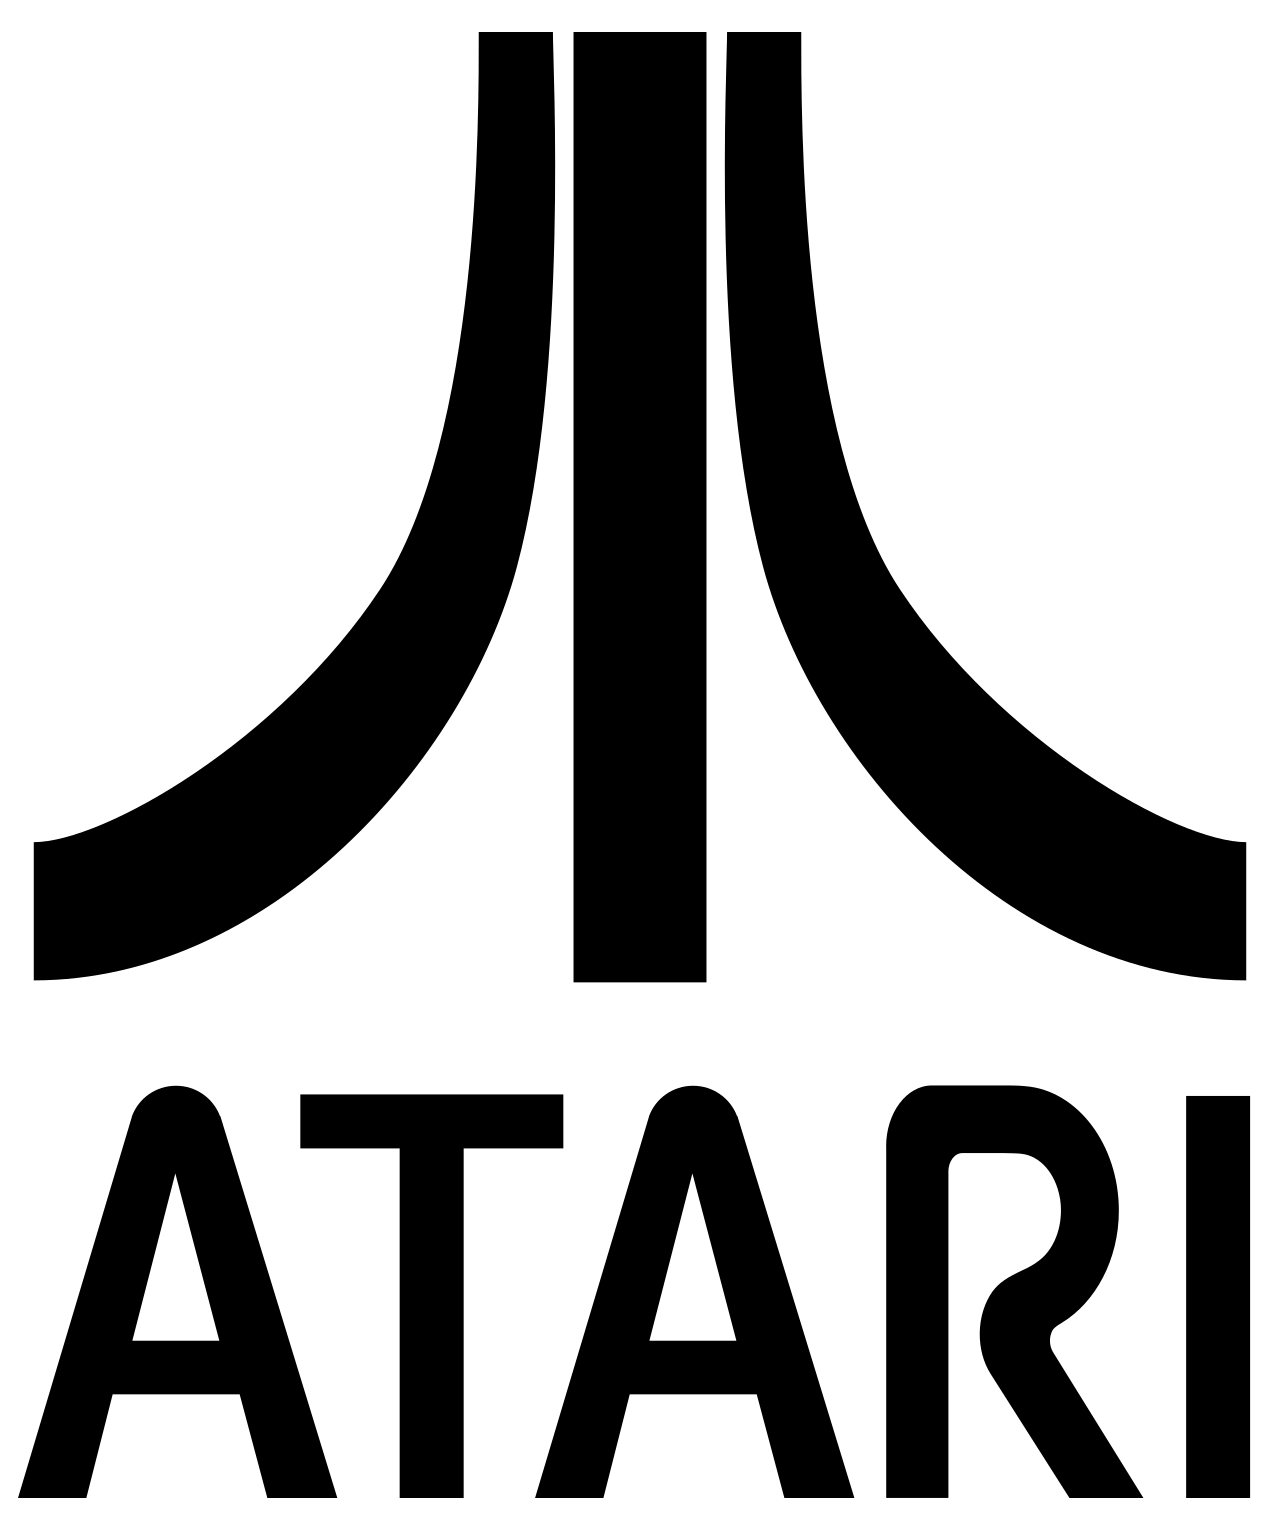
\includegraphics[width=1.8cm]{img/Atari.png}
        \caption{Atari-Logo}
      \end{figure}
      \vspace{-0.5cm}
     \begin{exampleblock}{Fun-Facts}
       \begin{itemize}
       \item Atari bez. eine Stellung in Go
       \item Steve Jobs/Wozniak arbeiteten vor der Gr\"undung von Apple bei Atari
       \end{itemize}
     \end{exampleblock}
    \end{minipage}
\end{frame}

%%%% Atari-Spiele %%%%
\begin{frame}
  \frametitle{Verschiedenste Spiele}
  \begin{minipage}{0.3\textwidth}
    \begin{adjustwidth}{}{}
      \begin{figure}[h!]
        \centering    
        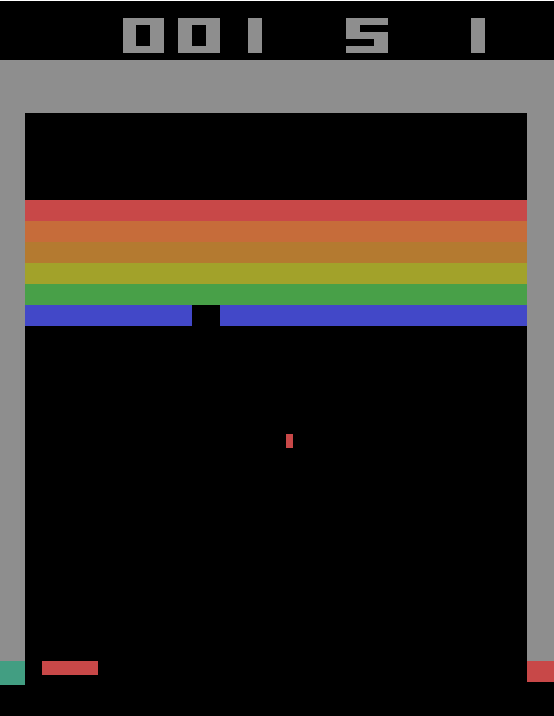
\includegraphics[width=2cm]{img/breakout.png} 
        \caption{Breakout}
      \end{figure}
    \end{adjustwidth}
    \begin{figure}[!h]
      \centering
      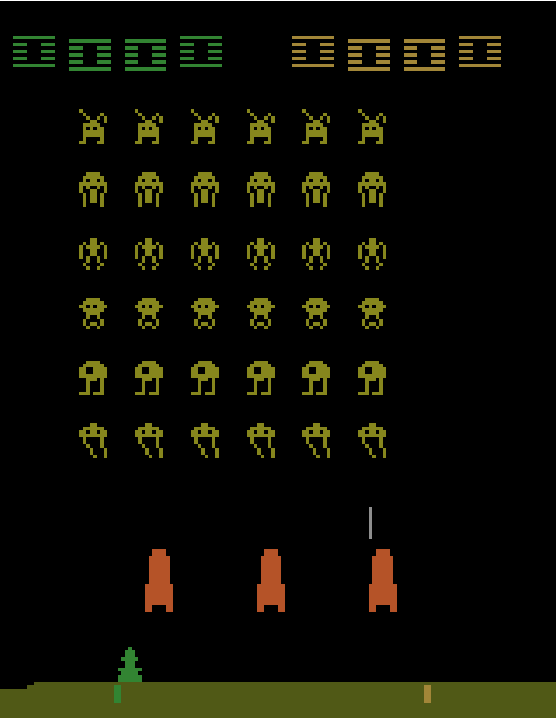
\includegraphics[width=2cm]{img/spaceinvader.png}
      \caption{SpaceInvaders}
    \end{figure}
  \end{minipage}
  \hfill
  \begin{minipage}{0.3\textwidth}
    \begin{adjustwidth}{-0.5cm}{}
      \begin{figure}
        \centering
        \includegraphics[width=3cm]{img/atari2600.png}
        \caption{Atari-2600}
      \end{figure}
    \end{adjustwidth}
    \vspace{0.5cm}
    \scriptsize{\boxed{$210\times160\times3$
    pixel}}
  \end{minipage}
  \begin{minipage}{0.3\textwidth}
    \begin{figure}[!h]
      \centering
      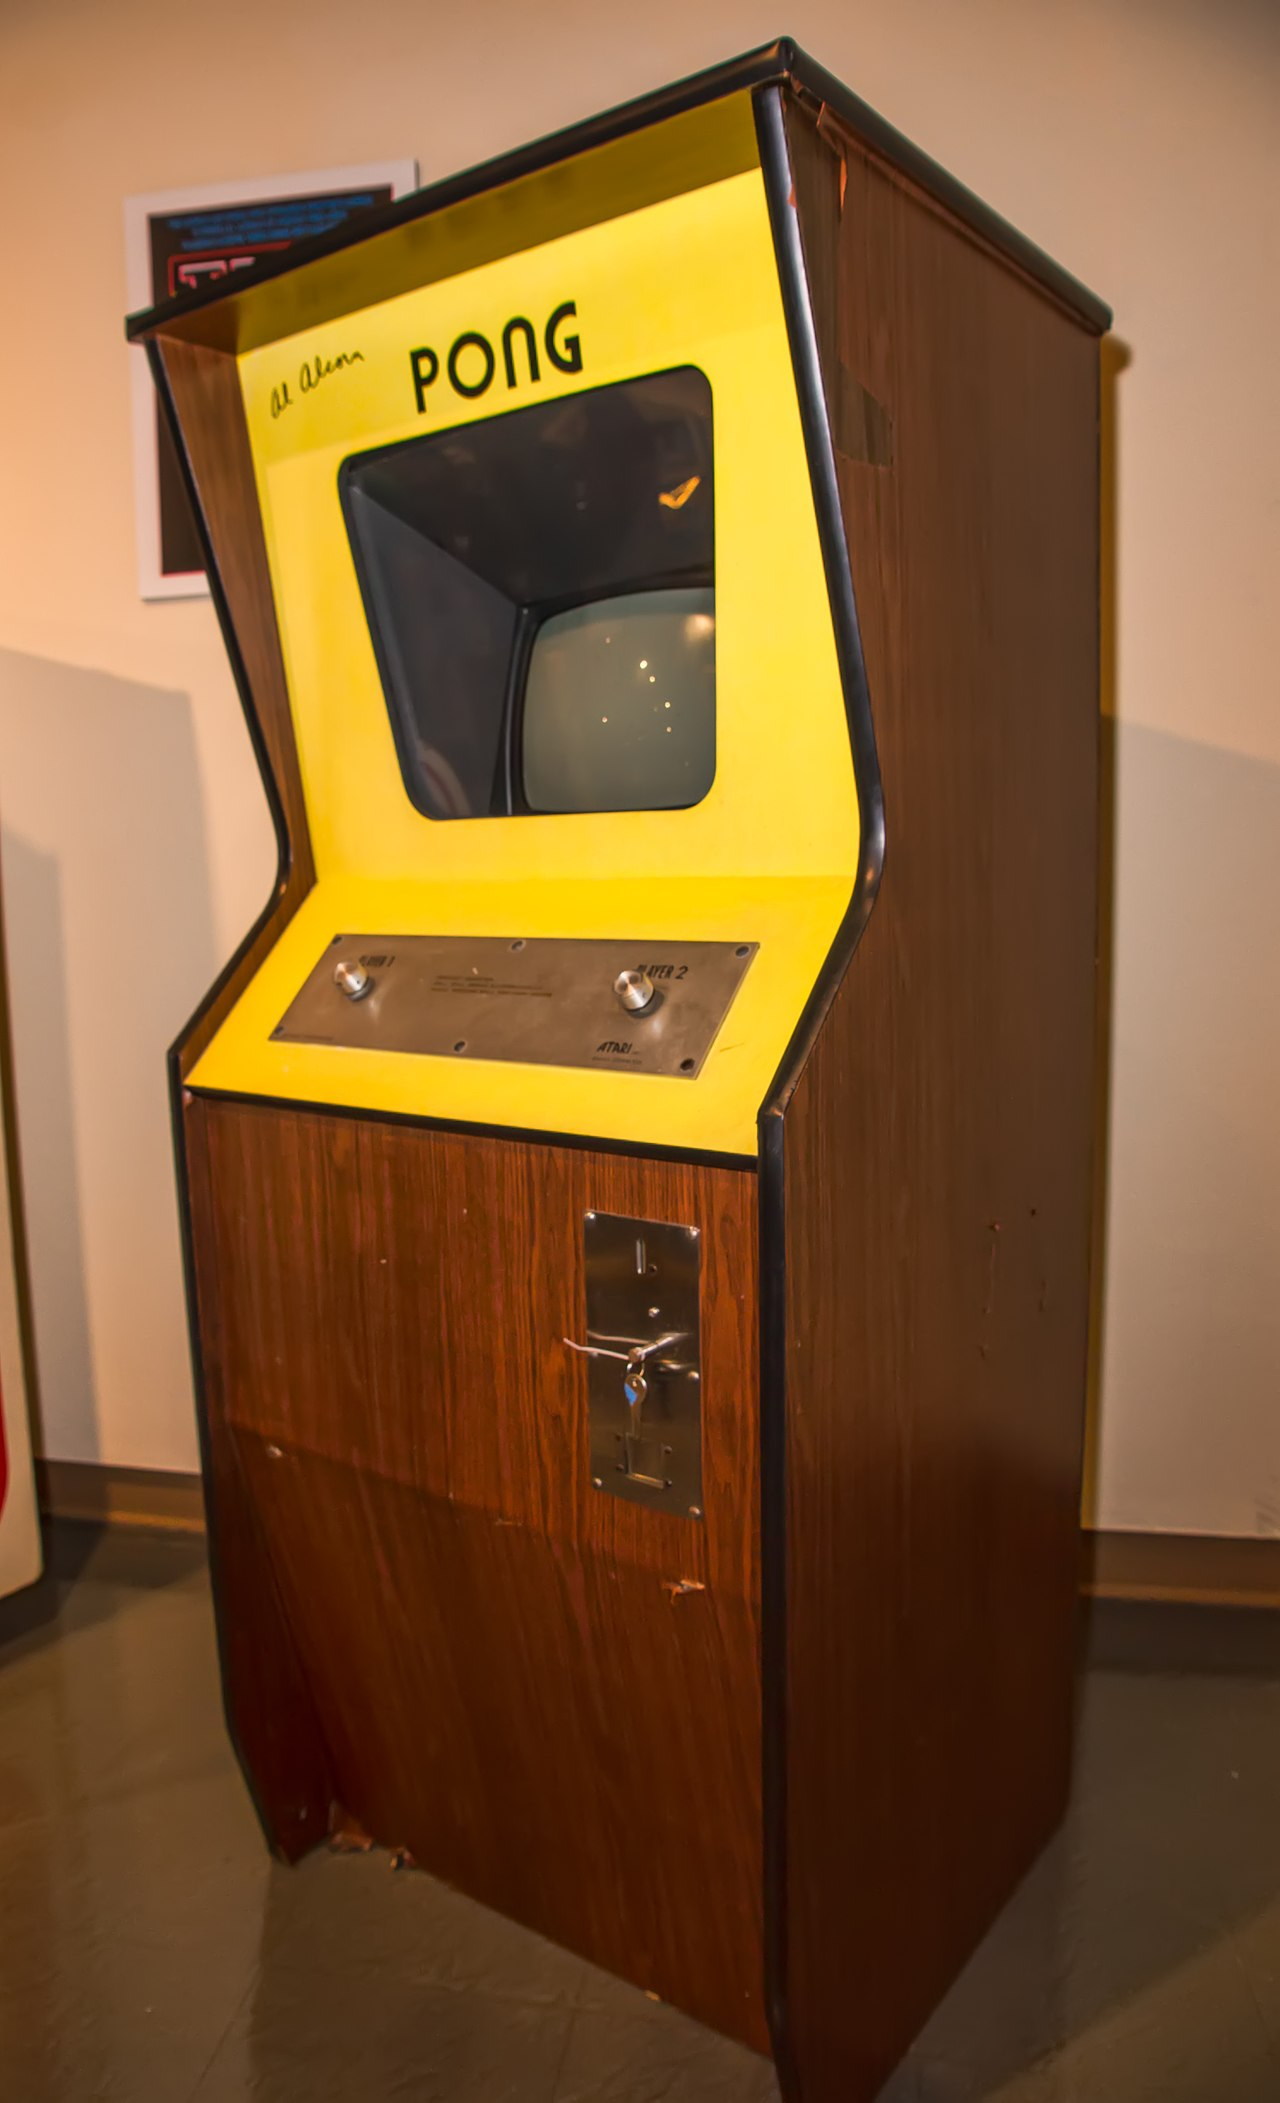
\includegraphics[width=2cm]{img/Pong.png}
      \caption{Pong}
    \end{figure}
    \vspace{-0.4cm}
      \begin{figure}[!h]
        \centering
        \includegraphics[width=2cm]{img/Pacman.png}
        \caption{Ms Pacman}
      \end{figure}
  \end{minipage}
\end{frame}

%%% 
\begin{frame}[fragile]
  \frametitle{Software/Benchmark-Sammlungen}
  \hspace{-0.2cm}
  \begin{minipage}{0.5\textwidth}
  \begin{lstlisting}[language=Python]
 from ale_py import ALEInterface
 ale = ALEInterface()
 ale.loadROM('Breakout')
  \end{lstlisting}
  \end{minipage}
  \hfill
  \begin{minipage}{0.5\textwidth}
    \begin{lstlisting}[language=Python]
 import gym
 env = gym.make('Breakout_v4')
 env.reset()
    \end{lstlisting}
  \end{minipage}
  \vspace{-0.4cm}
  \begin{block}{Arcade Learning Environment (2013)}
    Ein Herausforderndes Problem, eine Plattform und Testumgebung zur Bewertung und Vergleich von dom\"anenunabh\"angigen KI. 
    \begin{itemize}
    \item \"Uber 55 verschiedene Atari 2600 Spiele 
    \item Aufgebaut auf einem Open-Source Atari 2600 Emulator \textit{(Stella)}
    \end{itemize}
  \end{block}
  \vspace{-0.2cm}
  \begin{block}{OpenAI Gym (2016)}
    Versucht die besten Elemente vorheriger Benchmark-Sammlungen \textit{(ALE, RLLAB, \dots)} zu einem Software Paket zu vereinigen, das so bequem und zug\"anglich wie m\"oglich ist.
    \begin{itemize}
    \item Verschiedene Environments \textit{(MuJoCo, Robotics, \dots)}
    \end{itemize}
  \end{block}
\end{frame}

%%% 
\section{Problem}
\subsection{MDP}
\begin{frame}
  \frametitle{Houston, we have a problem}
  \vspace{-0.2cm}
  \begin{alertblock}{It's a Markov decision process}
    \begin{enumerate}
    \item Agent: \textit{maximiere zukunfts Belohnungen}
    \item Umgebung: $\mathcal{E}$
    \item Zustand: $\mathcal{S} = \{s_1,\dots,s_N\}$
    \item Aktion: $\mathcal{A} = \{a_1,\dots,a_N\}$
    \item Belohnung: $\mathcal{R} = \{r_1,\dots,r_N\}$
    \smash{\raisebox{.5\dimexpr1.9\baselineskip+4\itemsep+5\parskip}{$\left.\rule{0pt}{.4\dimexpr5\baselineskip+3\itemsep+5\parskip}\right\}\text{zu jedem Zeitpunkt } t-T$}}
    \end{enumerate}
  \end{alertblock}
  \vspace{-0.2cm}
  \pause
  \begin{block}{Sounds pretty simple}
    \begin{itemize}
    \item Umgebung $\rightarrow$ Atari-Emulator
    \item Zustand $\rightarrow$ Bild aus dem Emulator $x_t \in \mathbb{R}^d$ Vektor aus Pixeln
    \item Aktion $\rightarrow$ legale Spielaktionen (max. 18)
    \item Belohnung $\rightarrow$ \"Anderung des Spielstands
    \item Agent $\rightarrow$ max. zukunfts Belohnungen durch Interaktion mit dem Emulator
    \end{itemize}
  \end{block}
\end{frame}

\begin{frame}
  \frametitle{Spezifischer}
  \begin{block}{Zustand}
    Unm\"oglich das Spiel zu verstehen wenn wir ein Bild $x_t$ als Zustand nutzen. Daher nutzen wir eine Sequenz von Bildern und Aktionen $s_t = x_1,a_1,x_2,\dots,a_{t-1},x_t$. $\rightarrow$ Zustandsrepr\"asentation an Zeitpunkt $t$.
  \end{block}
  \pause
  \begin{block}{Belohnungen}
    Wir brauchen ein Ma� f\"ur die Belohnungen, z.B die max. zu holende Belohnungen in einer Episode \textit{(Punkt/Sterben)}. $R_t= \sum_{t^{'}=t}^{T}\gamma^{t^{'}-t}r_{t^{'}} \rightarrow$ return. Mit Erm\"a�igungsfaktor $0\leq\gamma\leq1$, hier $\gamma = 0.99$.
  \end{block}
\end{frame}

\subsection{Q-Funktionen}
\begin{frame}
  \frametitle{Q-Funktion}
  \vspace{-0.2cm}
  \begin{block}{Aktions-Wert Funktion}
    $$Q(s,a) = \mathbb{E}\left[R_t|s_t = s, a_t =a,\pi\right]$$ 
    Was ist der erwartete Return $R_t$, wenn wir in einem Zustand $s$ sind, Aktion $a$ ausf\"uhren und der Policy $\pi$ folgen. $\forall s \in \mathcal{S} \land \forall a \in \mathcal{A}(s)$,
  \end{block}
  \vspace{-0.2cm}
  \pause
  \begin{block}{Optimale Aktions-Wert Funktion}
    $$Q^{\ast}(s,a) = \max_{\pi}\mathbb{E}\left[R_t|s_t = s, a_t =a,\pi\right]$$
    Was ist der erwartete Return, wenn wir in $s$, $a$ ausf\"uhren und der optimalen policy $\pi^{\ast}$ folgen.
  \end{block}
  \vspace{-0.2cm}
  \begin{figure}[!h]
    \begin{columns}
      \hspace{1cm}
      \column{.0\linewidth}
      \begin{tikzpicture}
        \tikzstyle{sa} = [circle,draw,fill=black,inner sep=0pt,minimum width=3pt]
        \tikzstyle{s} = [circle,draw,inner sep=0pt,minimum width=5pt]
        \node(root)[sa,label=above:{\scriptsize{${s,a}$}}] at (2,1){};
        \node(a)[s] at (2,0.25){};
        \node(b)[s] at (1.25,0.25){};
        \node(c)[s,label=right:{\scriptsize{${s'}$}}] at (2.75,0.25){};
        \draw[->] (root) -- (a)node[left,yshift=0.3cm,xshift=0.1cm]{\scriptsize{${r_2}$}};;
        \draw[->] (root) -- (b)node[left,yshift=0.5cm,xshift=0.4cm]{\scriptsize{${r_1}$}};
        \draw[->] (root) -- (c)node[left,yshift=0.5cm,xshift=0.1cm]{\scriptsize{${r_3}$}};;
        \node(aa) [sa] at (2,-0.5);
        \node(ab) [sa] at (2.25,-0.5);
        \node(ac) [sa] at (1.75,-0.5);
        \draw[->,densely dotted] (a) -- (aa);
        \draw[->,densely dotted] (a) -- (ab);
        \draw[->,densely dotted] (a) -- (ac);
        \node(ba) [sa] at (1.5,-0.5);
        \node(bb) [sa] at (1.25,-0.5);
        \node(bc) [sa] at (1,-0.5);
        \draw[->,densely dotted] (b) -- (ba) node[left,xshift=-0.3cm,yshift=0.4cm]{\scriptsize{$\max$}};
        \draw[->,densely dotted] (b) -- (bb);
        \draw[->,densely dotted] (b) -- (bc);
        \node(ca) [sa] at (2.5,-0.5);
        \node(cb) [sa] at (2.75,-0.5);
        \node(cc) [sa] at (3,-0.5);
        \draw[->,densely dotted] (c) -- (ca);
        \draw[->,densely dotted] (c) -- (cb);
        \draw[->,densely dotted] (c) -- (cc) node[rigth,xshift=0.3cm,yshift=0.05cm]{\scriptsize{$a'$}};
      \end{tikzpicture}
      \column{.2\linewidth}
      \caption{Backup Diagramm $Q^{\ast}$}
    \end{columns}
  \end{figure}
\end{frame}


\begin{frame}
  \frametitle{Optimale Policy}
  \visible<1->{
    \begin{block}{Bellmann Gleichung}
      $$Q^{\ast}(s,a)=\mathbb{E}_{s'\sim\mathcal{E}}\left[r+\gamma\,\max_{a'}Q^{\ast}(s',a')\mid s,a\right]$$
  \end{block}}
  \visible<2->{
  \begin{minipage}{0.45\textwidth}
      \begin{figure}[!h]
        \centering
        
\includegraphics[width=4.5cm]{img/problem.png}
        \scriptsize{\caption*{\textbf{Quelle: } Randall Munroe, \url{https://xkcd.com/1739/}}}
      \end{figure}
  \end{minipage}
  \hfill
  \begin{minipage}{0.45\textwidth}
    \vspace{-1cm}
    \centering Wie finden wir $Q^{\ast}$ und somit eine optimale Policy $\pi^\ast$ f\"ur unseren Agent ?
    \end{minipage}}
\end{frame}


\section{Model}
\subsection{Q-Netzwerk}
\begin{frame}
  \frametitle{Q-Netzwerk}
  \centering
  Wir erstellen ein K\"unstliches Neuronales Netz und versuchen somit $Q^{\ast}$ zu approximieren.
    $$Q(s,a;\theta) \approx Q^{\ast}(s,a)$$
  \pause
  \centering
  Das machen wir mit Hilfe einer Verlustfunktion.
  \begin{tcolorbox}[colframe=red!50]
  $$\mathcal{L}_{i}(\theta_i)=\mathbb{E}_{s,a\sim p(\cdot)}\left[(y_i-Q(s,a,\theta_i))^2\right]$$
  \end{tcolorbox}
  mit dem Ziel $y_i = \mathbb{E}_{s'\sim \mathcal{E}}\left[r+\gamma\max_{a'}Q(s',a';\theta_{i-1})\right\mid s,a]$ f\"ur jede Interation, versuchen wir diese Verlustfunktion durch einen Gradientenverfahren zu minimieren und so $Q^{\ast}$ zu approximieren.\\ \vspace{0.3cm}
  \pause
  \centering
  \textcolor{red}{Um welche Verlustfunktion handelt es sich in dieser Formel ?} \\
  \visible<4->{L2-Verlustfunktion}
\end{frame}

\subsection{Architektur}
\begin{frame}
  \frametitle{Q-Netzwerk/Architektur}
  \begin{figure}[!h]
    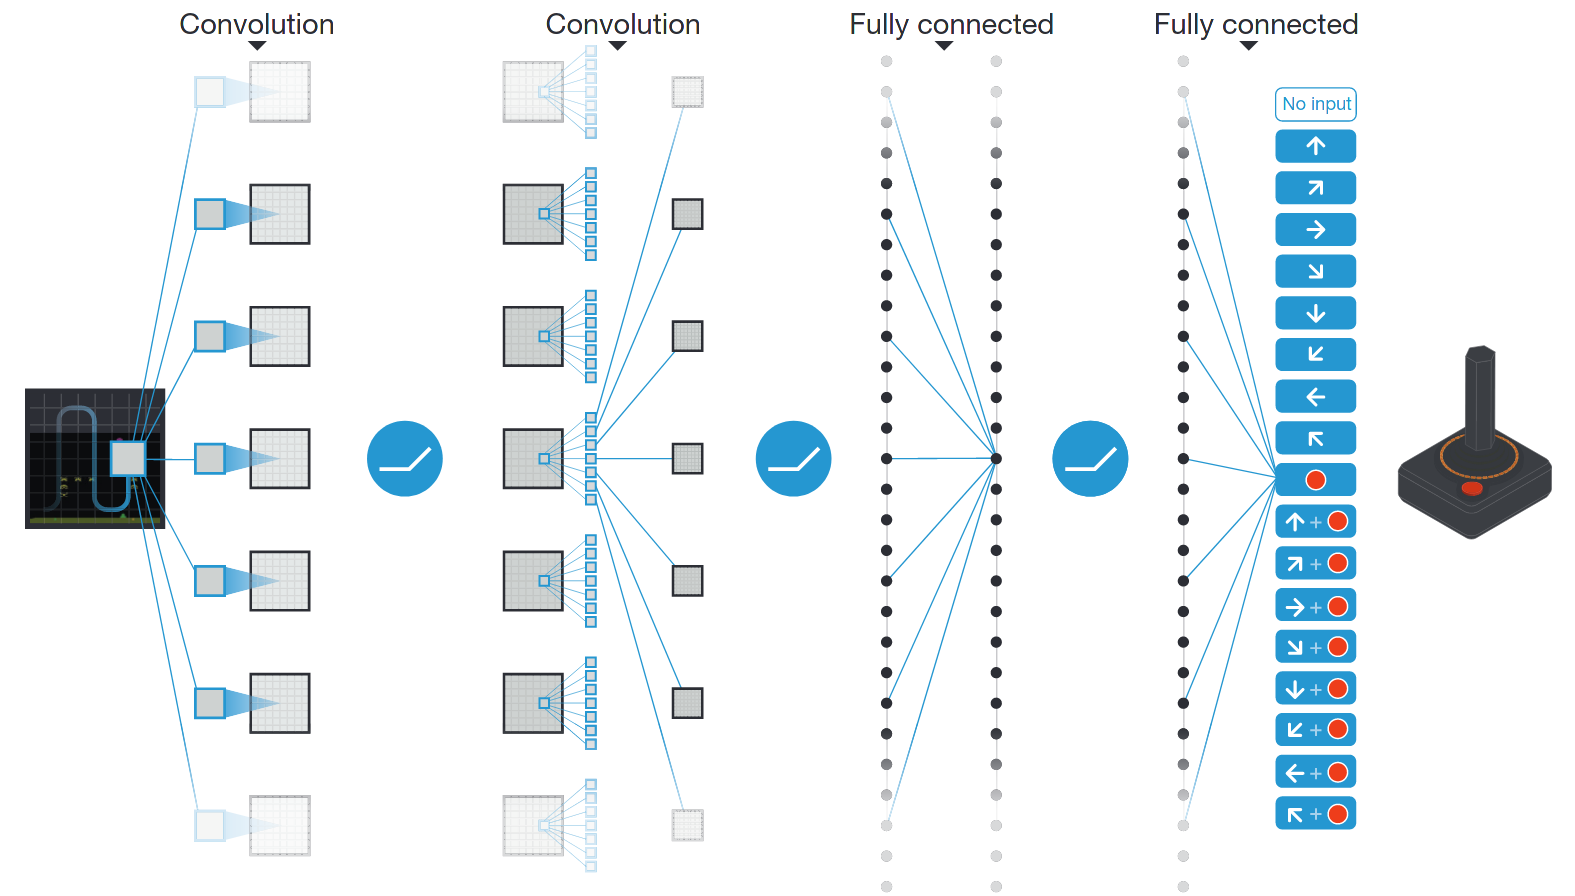
\includegraphics[width=7cm]{img/A.png}
    \scriptsize{\caption*{\textbf{Quelle:} V. Mnih, \url{https://www.nature.com/articles/nature14236}}}
  \end{figure}
  \vspace{-0.4cm}
  \centering
  \scriptsize{
    \begin{tabular}{|c|| c ||c |}
      \hline
      \textbf{Schicht} & \textbf{Details} & \textbf{Aktivierung} \\
      \hline\hline
      Eingabe & ($84\times84\times4$) Eingabe durch $\phi(s)$ & \\
      Faltung & 16 ($8\times8$) Filter, Schritt 4 & ReLU \\
      Faltung & 32 ($4\times4$) Filter, Schritt 2 & ReLU \\
      Dense & 256 verborgene Neuronen & ReLU \\
      Dense (Ausgabe) & Ein Neuron pro Aktion & Linear\\
      \hline
    \end{tabular}
  }
\end{frame}

\begin{frame}
  \frametitle{Vorverarbeitung}
  \vspace{-0.2cm}
  \begin{block}{Was ist nun $\phi(s)$}
    Ein Vorverarbeitungsschritt um Eingabedimensionen zu reduzieren. Durch RGB zu Grauskalierung und komprimieren des Bildes.
    \begin{itemize}
    \item $210 \times 160 \times 3  \rightarrow 110 \times 84 \times 1$
    \end{itemize}
  \end{block}
  \vspace{-0.2cm}
  \begin{alertblock}{Can we do better ?}
    Interessant ist die Spielfl\"ache, also schneiden wir sie aus dem Bild.
    \begin{itemize}
    \item $84\times84\times1$, jedoch stapeln wir vier davon hintereinander $\times 4$. 
    \end{itemize}
  \end{alertblock}
  \hspace{-0.3cm}
  \begin{minipage}{0.7\textwidth}
    \begin{figure}[!h]
      \centering
      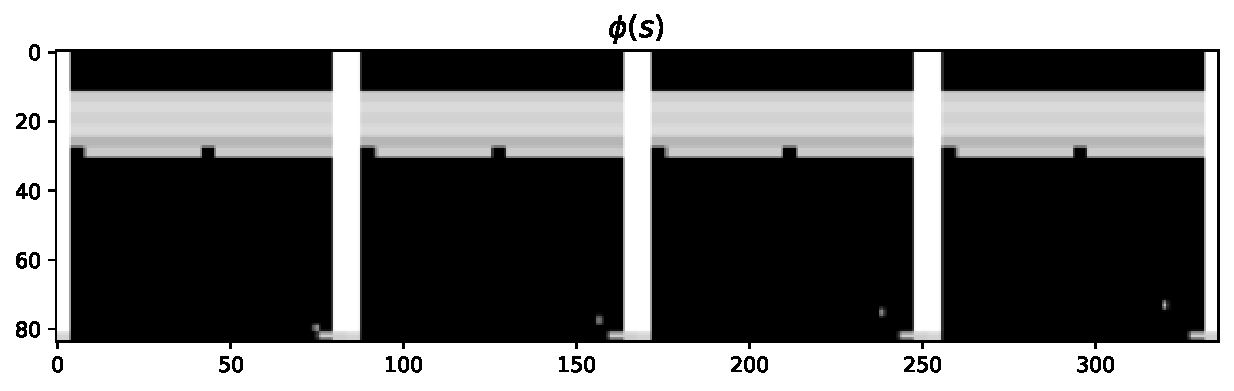
\includegraphics[width=8cm]{img/phi.pdf}
      \caption{$\phi(s)$: Input Q-Netzwerk}
    \end{figure}
  \end{minipage}
  \hfill
  \begin{minipage}{0.3\textwidth}
    \begin{adjustwidth}{}{}
      \begin{figure}[!h]
        \centering
        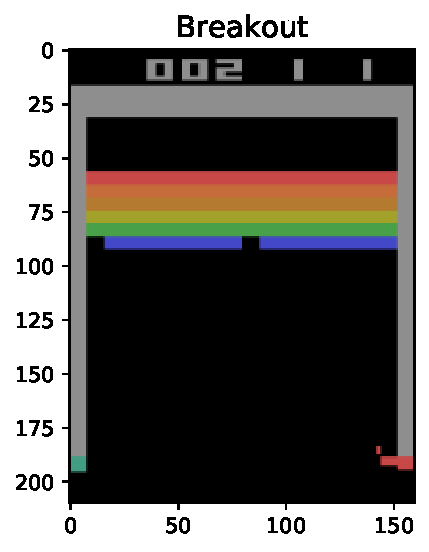
\includegraphics[width=1.8cm]{img/breakout.pdf}
        \caption{Breakout}
      \end{figure}
    \end{adjustwidth}
  \end{minipage}
\end{frame}

\begin{frame}[fragile]
  \frametitle{Faltung/CNN}
  \centering Filter $4\times4$ \\
  \begin{figure}[!h]
    \centering
    \begin{tikzpicture}
      \usetikzlibrary{matrix}
      \begin{onlyenv}<1>
      \matrix (mtr) [matrix of nodes,row sep=-\pgflinewidth, nodes={draw}]
	{
		|[fill=red!30]| 1 & |[fill=red!30]| 0 & |[fill=red!30]| 0 & |[fill=red!30]| 0 & 0 & 1 & 1 & 0\\
		|[fill=red!30]| 1 & |[fill=red!30]| 1 & |[fill=red!30]| 0 & |[fill=red!30]| 0 & 0 & 0 & 1 & 1\\
		|[fill=red!30]| 1 & |[fill=red!30]| 1 & |[fill=red!30]| 1 & |[fill=red!30]| 0 & 0 & 0 & 0 & 1\\
		|[fill=red!30]| 0 & |[fill=red!30]| 0 & |[fill=red!30]| 0 & |[fill=red!30]| 1 & 1 & 0 & 0 & 1\\
		0 & 0 & 1 & 1 & 0 & 0 & 0 & 1\\
		0 & 1 & 1 & 0 & 0 & 0 & 0 & 1\\
        0 & 0 & 1 & 1 & 0 & 0 & 0 & 1\\
	};
	\draw[very thick, red] (mtr-1-1.north west) rectangle (mtr-4-4.south east); %

	\node [below= of mtr-5-4.south,xshift=0.2cm] (lm) {$\bf \boldsymbol{\phi}(s)$};

	\node[right = 0.2em of mtr] (str) {$*$};

	\matrix (K) [right=0.2em of str,matrix of nodes,row sep=-\pgflinewidth, nodes={draw, fill=blue!30}]
	{
		1 & 0 & 0 & 0\\
		0 & 1 & 0 & 0\\
		0 & 0 & 1 & 0\\
        0 & 0 & 0 & 1\\
	};
	\node [below = of K-3-2.south,xshift=0.25cm,yshift=0.4cm] (lk) {$\bf 4\times4 $};

	\node [right = 0.2em of K] (eq) {$=$};
	\matrix (ret) [right=0.2em of eq,matrix of nodes,row sep=-\pgflinewidth, nodes={draw}]
	{
		1 & 4 & 3 & |[fill=green!30]| 4 & 1\\
		1 & 2 & 4 & 3 & 3\\
		1 & 2 & 3 & 4 & 1\\
		1 & 3 & 3 & 1 & 1\\
		3 & 3 & 1 & 1 & 0\\
	};
	\node [below = of ret-4-3.south,yshift=0.3cm] (lim) {Output};

	\draw[very thick, green] (ret-1-4.north west) rectangle (ret-1-4.south east);

	\draw[densely dotted, blue, thick] (mtr-1-1.north west) -- (K-1-1.north west);
	\draw[densely dotted, blue, thick] (mtr-4-1.south west) -- (K-4-1.south west);
	\draw[densely dotted, blue, thick] (mtr-1-4.north east) -- (K-1-4.north east);
	\draw[densely dotted, blue, thick] (mtr-4-4.south east) -- (K-4-4.south east);

	\draw[densely dotted, green, thick] (ret-1-4.north west) -- (K-1-1.north west);
	\draw[densely dotted, green, thick] (ret-1-4.south west) -- (K-4-1.south west);
	\draw[densely dotted, green, thick] (ret-1-4.north east) -- (K-1-4.north east);
	\draw[densely dotted, green, thick] (ret-1-4.south east) -- (K-4-4.south east);

	\matrix (K) [right=0.2em of str,matrix of nodes,row sep=-\pgflinewidth, nodes={draw, fill=blue!10}]
	{
	    1 & 0 & 0 & 0\\
		0 & 1 & 0 & 0\\
		0 & 0 & 1 & 0\\
        0 & 0 & 0 & 1\\
	};

	\draw[very thick, blue] (K-1-1.north west) rectangle (K-4-4.south east);
    %
	\node[anchor=south east, inner sep=0.01em, blue] at (mtr-1-1.south east) (xx) {\scalebox{.5}{$\times 1$}};
	\node[anchor=south east, inner sep=0.01em, blue] at (mtr-1-2.south east) (xx) {\scalebox{.5}{$\times 0$}};
	\node[anchor=south east, inner sep=0.01em, blue] at (mtr-1-3.south east) (xx) {\scalebox{.5}{$\times 0$}};
    \node[anchor=south east, inner sep=0.01em, blue] at (mtr-1-4.south east) (xx) {\scalebox{.5}{$\times 0$}};
	\node[anchor=south east, inner sep=0.01em, blue] at (mtr-2-1.south east) (xx) {\scalebox{.5}{$\times 0$}};
	\node[anchor=south east, inner sep=0.01em, blue] at (mtr-2-2.south east) (xx) {\scalebox{.5}{$\times 1$}};
	\node[anchor=south east, inner sep=0.01em, blue] at (mtr-2-3.south east) (xx) {\scalebox{.5}{$\times 0$}};
    \node[anchor=south east, inner sep=0.01em, blue] at (mtr-2-4.south east) (xx) {\scalebox{.5}{$\times 0$}};
	\node[anchor=south east, inner sep=0.01em, blue] at (mtr-3-1.south east) (xx) {\scalebox{.5}{$\times 0$}};
	\node[anchor=south east, inner sep=0.01em, blue] at (mtr-3-2.south east) (xx) {\scalebox{.5}{$\times 0$}};
	\node[anchor=south east, inner sep=0.01em, blue] at (mtr-3-3.south east) (xx) {\scalebox{.5}{$\times 1$}};
    \node[anchor=south east, inner sep=0.01em, blue] at (mtr-3-4.south east) (xx) {\scalebox{.5}{$\times 0$}};
    \node[anchor=south east, inner sep=0.01em, blue] at (mtr-4-1.south east) (xx) {\scalebox{.5}{$\times 0$}};
    \node[anchor=south east, inner sep=0.01em, blue] at (mtr-4-2.south east) (xx) {\scalebox{.5}{$\times 0$}};
    \node[anchor=south east, inner sep=0.01em, blue] at (mtr-4-3.south east) (xx) {\scalebox{.5}{$\times 0$}};
    \node[anchor=south east, inner sep=0.01em, blue] at (mtr-4-4.south east) (xx) {\scalebox{.5}{$\times 1$}};
      \end{onlyenv}
      %%%Second Slide%%%
      \begin{onlyenv}<2>
        \matrix (mtr) [matrix of nodes,row sep=-\pgflinewidth, nodes={draw}]
	{
		1 & 0 & |[fill=red!30]| 0 & |[fill=red!30]| 0 & |[fill=red!30]| 0 & |[fill=red!30]| 1 & 1 & 0\\
		1 & 1 & |[fill=red!30]| 0 & |[fill=red!30]| 0 & |[fill=red!30]| 0 & |[fill=red!30]| 0 & 1 & 1\\
		1 & 1 & |[fill=red!30]| 1 & |[fill=red!30]| 0 & |[fill=red!30]| 0 & |[fill=red!30]| 0 & 0 & 1\\
		0 & 0 & |[fill=red!30]| 0 & |[fill=red!30]| 1 & |[fill=red!30]| 1 & |[fill=red!30]| 0 & 0 & 1\\
		0 & 0 & 1 & 1 & 0 & 0 & 0 & 1\\
		0 & 1 & 1 & 0 & 0 & 0 & 0 & 1\\
        0 & 0 & 1 & 1 & 0 & 0 & 0 & 1\\
	};
	\draw[very thick, red] (mtr-1-3.north west) rectangle (mtr-4-6.south east); %

	\node [below= of mtr-5-4.south,xshift=0.2cm] (lm) {$\bf \boldsymbol{\phi}(s)$};
    \node [above= of mtr-3-4.north] (stride) {\scriptsize{$\bf schritt=2 \rightarrow$}};
	\node[right = 0.2em of mtr] (str) {$*$};
    
	\matrix (K) [right=0.2em of str,matrix of nodes,row sep=-\pgflinewidth, nodes={draw, fill=blue!30}]
	{
		1 & 0 & 0 & 0\\
		0 & 1 & 0 & 0\\
		0 & 0 & 1 & 0\\
        0 & 0 & 0 & 1\\
	};
	\node [below = of K-3-2.south,xshift=0.25cm,yshift=0.4cm] (lk) {$\bf 4\times4 $};

	\node [right = 0.2em of K] (eq) {$=$};
	\matrix (ret) [right=0.2em of eq,matrix of nodes,row sep=-\pgflinewidth, nodes={draw}]
	{
		1 & 4 & 3 & |[fill=green!30]| 4 & 1\\
		1 & 2 & 4 & 3 & 3\\
		1 & 2 & 3 & 4 & 1\\
		1 & 3 & 3 & 1 & 1\\
		3 & 3 & 1 & 1 & 0\\
	};
	\node [below = of ret-4-3.south,yshift=0.3cm] (lim) {Output};
    
	\draw[very thick, green] (ret-1-4.north west) rectangle (ret-1-4.south east);

	\draw[densely dotted, blue, thick] (mtr-1-3.north west) -- (K-1-1.north west);
	\draw[densely dotted, blue, thick] (mtr-4-3.south west) -- (K-4-1.south west);
	\draw[densely dotted, blue, thick] (mtr-1-6.north east) -- (K-1-4.north east);
	\draw[densely dotted, blue, thick] (mtr-4-6.south east) -- (K-4-4.south east);

    
	\draw[densely dotted, green, thick] (ret-1-4.north west) -- (K-1-1.north west);
	\draw[densely dotted, green, thick] (ret-1-4.south west) -- (K-4-1.south west);
	\draw[densely dotted, green, thick] (ret-1-4.north east) -- (K-1-4.north east);
	\draw[densely dotted, green, thick] (ret-1-4.south east) -- (K-4-4.south east);
    
	\matrix (K) [right=0.2em of str,matrix of nodes,row sep=-\pgflinewidth, nodes={draw, fill=blue!10}]
	{
	    1 & 0 & 0 & 0\\
		0 & 1 & 0 & 0\\
		0 & 0 & 1 & 0\\
        0 & 0 & 0 & 1\\
	};
    
	\draw[very thick, blue] (K-1-1.north west) rectangle (K-4-4.south east);
    %
	\node[anchor=south east, inner sep=0.01em, blue] at (mtr-1-3.south east) (xx) {\scalebox{.5}{$\times 1$}};
	\node[anchor=south east, inner sep=0.01em, blue] at (mtr-1-4.south east) (xx) {\scalebox{.5}{$\times 0$}};
	\node[anchor=south east, inner sep=0.01em, blue] at (mtr-1-5.south east) (xx) {\scalebox{.5}{$\times 0$}};
    \node[anchor=south east, inner sep=0.01em, blue] at (mtr-1-6.south east) (xx) {\scalebox{.5}{$\times 0$}};
	\node[anchor=south east, inner sep=0.01em, blue] at (mtr-2-3.south east) (xx) {\scalebox{.5}{$\times 0$}};
	\node[anchor=south east, inner sep=0.01em, blue] at (mtr-2-4.south east) (xx) {\scalebox{.5}{$\times 1$}};
	\node[anchor=south east, inner sep=0.01em, blue] at (mtr-2-5.south east) (xx) {\scalebox{.5}{$\times 0$}};
    \node[anchor=south east, inner sep=0.01em, blue] at (mtr-2-6.south east) (xx) {\scalebox{.5}{$\times 0$}};
	\node[anchor=south east, inner sep=0.01em, blue] at (mtr-3-3.south east) (xx) {\scalebox{.5}{$\times 0$}};
	\node[anchor=south east, inner sep=0.01em, blue] at (mtr-3-4.south east) (xx) {\scalebox{.5}{$\times 0$}};
	\node[anchor=south east, inner sep=0.01em, blue] at (mtr-3-5.south east) (xx) {\scalebox{.5}{$\times 1$}};
    \node[anchor=south east, inner sep=0.01em, blue] at (mtr-3-6.south east) (xx) {\scalebox{.5}{$\times 0$}};
    \node[anchor=south east, inner sep=0.01em, blue] at (mtr-4-3.south east) (xx) {\scalebox{.5}{$\times 0$}};
    \node[anchor=south east, inner sep=0.01em, blue] at (mtr-4-4.south east) (xx) {\scalebox{.5}{$\times 0$}};
    \node[anchor=south east, inner sep=0.01em, blue] at (mtr-4-5.south east) (xx) {\scalebox{.5}{$\times 0$}};
    \node[anchor=south east, inner sep=0.01em, blue] at (mtr-4-6.south east) (xx) {\scalebox{.5}{$\times 1$}};
      \end{onlyenv}
      %%%3-Slide%%%
      \begin{onlyenv}<3>
         \matrix (mtr) [matrix of nodes,row sep=-\pgflinewidth, nodes={draw}]
	{
		1 & 0 & |[fill=red!30]| 0 & |[fill=red!30]| 0 & |[fill=red!30]| 0 & |[fill=red!30]| 1 & 1 & 0\\
		1 & 1 & |[fill=red!30]| 0 & |[fill=red!30]| 0 & |[fill=red!30]| 0 & |[fill=red!30]| 0 & 1 & 1\\
		1 & 1 & |[fill=red!30]| 1 & |[fill=red!30]| 0 & |[fill=red!30]| 0 & |[fill=red!30]| 0 & 0 & 1\\
		0 & 0 & |[fill=red!30]| 0 & |[fill=red!30]| 1 & |[fill=red!30]| 1 & |[fill=red!30]| 0 & 0 & 1\\
		0 & 0 & 1 & 1 & 0 & 0 & 0 & 1\\
		0 & 1 & 1 & 0 & 0 & 0 & 0 & 1\\
        0 & 0 & 1 & 1 & 0 & 0 & 0 & 1\\
	};
	\draw[very thick, red] (mtr-1-3.north west) rectangle (mtr-4-6.south east); %

	\node [below= of mtr-5-4.south,xshift=0.2cm] (lm) {$\bf \boldsymbol{\phi}(s)$};

	\node[right = 0.2em of mtr] (str) {$*$};

	\matrix (K) [right=0.2em of str,matrix of nodes,row sep=-\pgflinewidth, nodes={draw, fill=blue!30}]
	{
		1 & 0 & 0 & 0\\
		0 & 1 & 0 & 0\\
		0 & 0 & 1 & 0\\
        0 & 0 & 0 & 1\\
	};
	\node [below = of K-3-2.south,xshift=0.25cm,yshift=0.4cm] (lk) {$\bf 4\times4 $};

	\node [right = 0.2em of K] (eq) {$=$};
	\matrix (ret) [right=0.2em of eq,matrix of nodes,row sep=-\pgflinewidth, nodes={draw}]
	{
		1 & 4 & 3 & 4 & |[fill=green!30]| 0\\
		1 & 2 & 4 & 3 & 3\\
		1 & 2 & 3 & 4 & 1\\
		1 & 3 & 3 & 1 & 1\\
		3 & 3 & 1 & 1 & 0\\
	};
	\node [below = of ret-4-3.south,yshift=0.3cm] (lim) {Output};

	\draw[very thick, green] (ret-1-5.north west) rectangle (ret-1-5.south east);

	\draw[densely dotted, blue, thick] (mtr-1-3.north west) -- (K-1-1.north west);
	\draw[densely dotted, blue, thick] (mtr-4-3.south west) -- (K-4-1.south west);
	\draw[densely dotted, blue, thick] (mtr-1-6.north east) -- (K-1-4.north east);
	\draw[densely dotted, blue, thick] (mtr-4-6.south east) -- (K-4-4.south east);

    
	\draw[densely dotted, green, thick] (ret-1-5.north west) -- (K-1-1.north west);
	\draw[densely dotted, green, thick] (ret-1-5.south west) -- (K-4-1.south west);
	\draw[densely dotted, green, thick] (ret-1-5.north east) -- (K-1-4.north east);
	\draw[densely dotted, green, thick] (ret-1-5.south east) -- (K-4-4.south east);
    
	\matrix (K) [right=0.2em of str,matrix of nodes,row sep=-\pgflinewidth, nodes={draw, fill=blue!10}]
	{
	    1 & 0 & 0 & 0\\
		0 & 1 & 0 & 0\\
		0 & 0 & 1 & 0\\
        0 & 0 & 0 & 1\\
	};
    
	\draw[very thick, blue] (K-1-1.north west) rectangle (K-4-4.south east);
    %
	\node[anchor=south east, inner sep=0.01em, blue] at (mtr-1-3.south east) (xx) {\scalebox{.5}{$\times 1$}};
	\node[anchor=south east, inner sep=0.01em, blue] at (mtr-1-4.south east) (xx) {\scalebox{.5}{$\times 0$}};
	\node[anchor=south east, inner sep=0.01em, blue] at (mtr-1-5.south east) (xx) {\scalebox{.5}{$\times 0$}};
    \node[anchor=south east, inner sep=0.01em, blue] at (mtr-1-6.south east) (xx) {\scalebox{.5}{$\times 0$}};
	\node[anchor=south east, inner sep=0.01em, blue] at (mtr-2-3.south east) (xx) {\scalebox{.5}{$\times 0$}};
	\node[anchor=south east, inner sep=0.01em, blue] at (mtr-2-4.south east) (xx) {\scalebox{.5}{$\times 1$}};
	\node[anchor=south east, inner sep=0.01em, blue] at (mtr-2-5.south east) (xx) {\scalebox{.5}{$\times 0$}};
    \node[anchor=south east, inner sep=0.01em, blue] at (mtr-2-6.south east) (xx) {\scalebox{.5}{$\times 0$}};
	\node[anchor=south east, inner sep=0.01em, blue] at (mtr-3-3.south east) (xx) {\scalebox{.5}{$\times 0$}};
	\node[anchor=south east, inner sep=0.01em, blue] at (mtr-3-4.south east) (xx) {\scalebox{.5}{$\times 0$}};
	\node[anchor=south east, inner sep=0.01em, blue] at (mtr-3-5.south east) (xx) {\scalebox{.5}{$\times 1$}};
    \node[anchor=south east, inner sep=0.01em, blue] at (mtr-3-6.south east) (xx) {\scalebox{.5}{$\times 0$}};
    \node[anchor=south east, inner sep=0.01em, blue] at (mtr-4-3.south east) (xx) {\scalebox{.5}{$\times 0$}};
    \node[anchor=south east, inner sep=0.01em, blue] at (mtr-4-4.south east) (xx) {\scalebox{.5}{$\times 0$}};
    \node[anchor=south east, inner sep=0.01em, blue] at (mtr-4-5.south east) (xx) {\scalebox{.5}{$\times 0$}};
    \node[anchor=south east, inner sep=0.01em, blue] at (mtr-4-6.south east) (xx) {\scalebox{.5}{$\times 1$}}
      \end{onlyenv}
    \end{tikzpicture}
  \end{figure}
\end{frame}

\subsection{DQN-Algorithmus}
\begin{frame}[fragile]
  \frametitle{Algoritmus}
  \begin{block}{Deep Q-Learning mit Erlebnis-Wiedergabe}
    \scriptsize{
    \begin{algorithm}
      \label{DQN}\begin{algorithmic}[1]
        \State Initialisiere Wiedergabespeicher $\mathcal{D}$ mit Kapazit\"at $N$
        \State Initialisiere aktions-werte Funktion $Q$ mit zuf\"alligen Gewichten
        \For{Episode = 1,$M$}
        \State Initialisiere Sequenz $s_1$ = \{$x_1$\} und vorverarbeite $\phi_1(s) = \phi(s_1)$
        \For{$t=1,T$}
        \State Mit Wahrscheinlichkeit $\epsilon$ w\"ahle eine zuf�llige Aktion $a_t$
        \State andernfalls w\"ahle $a_t =\max_a Q(\phi(s_t),a;\theta)$
        \State F�hre Aktion $a_t$ im Emulator aus, erhalte Belohnung $r_t$ und Bild $x_{t+1}$
        \State Setze $s_{t+1} = s_t,a_t,x_{t+1}$ und vorverarbeite $\phi_{t+1} = \phi(s_{t+1})$
        \State Speicher \"Ubergang ($\phi_t,a_t,r_t,\phi_{t+1}$) in $\mathcal{D}$
        \State W\"ahle einen zuf\"alligen minibatch von \"Uberg\"angen ($\phi_j,a_j,r_j,\phi_{j+1}$) aus $\mathcal{D}$
        \State Setze $y_i =$ \begin{cases} r_j & \quad \text{f\"ur beendendes}\,\, \phi_{j+1} \\
          r_j+\gamma\max_{a'}Q(\phi_{j+1},a';\theta) & \quad \text{f\"ur nicht beendendes}\,\, \phi_{j+1} \end{cases}
        \State Mache einen Gradientenabstieg schritt auf $(y_j-Q(\phi_j,a_j;\theta))^2$
        \EndFor
        \EndFor
      \end{algorithmic}
    \end{algorithm}
    }
  \end{block}
\end{frame}

\subsection{Ergebnisse}
\begin{frame}%%%
  \hspace{-0.5cm}
  \begin{minipage}{0.45\textwidth}
    \frametitle{Ergebnisse aus 2015}
  \begin{figure}[!h]
    \centering
    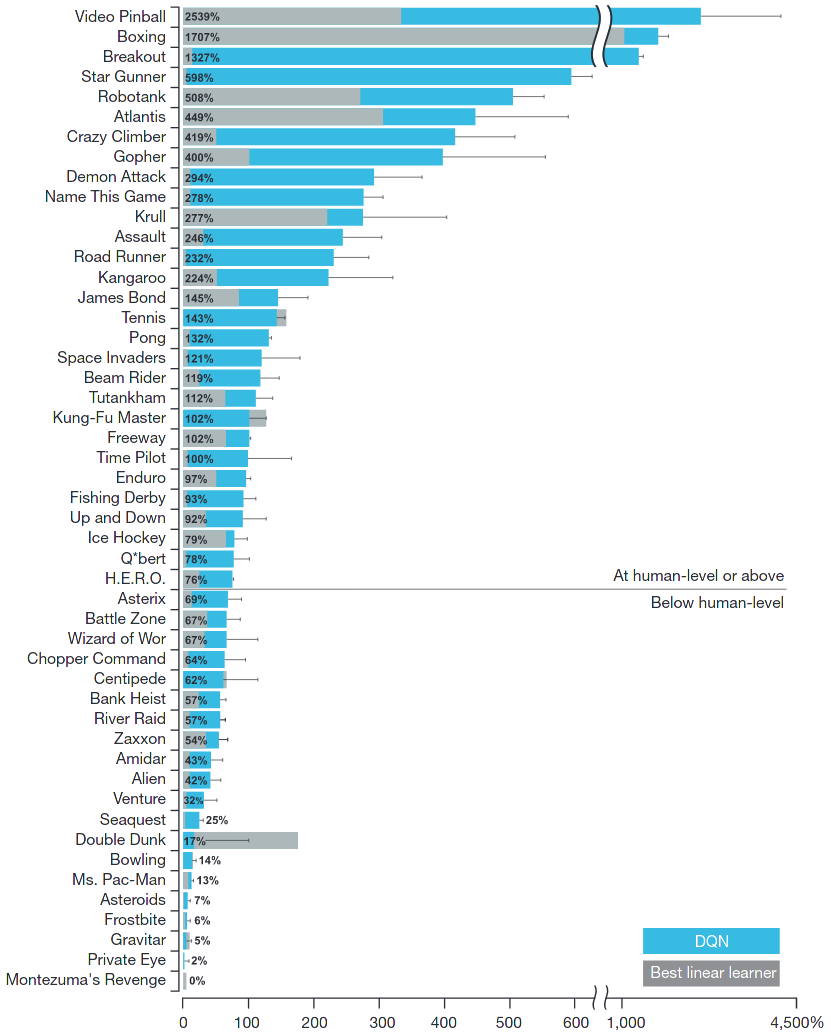
\includegraphics[width=5.8cm]{img/Ergebnisse.png}
  \end{figure}
  \end{minipage}
  \hfill
  \begin{minipage}{0.45\textwidth}
    \begin{figure}[!h]
      \centering
      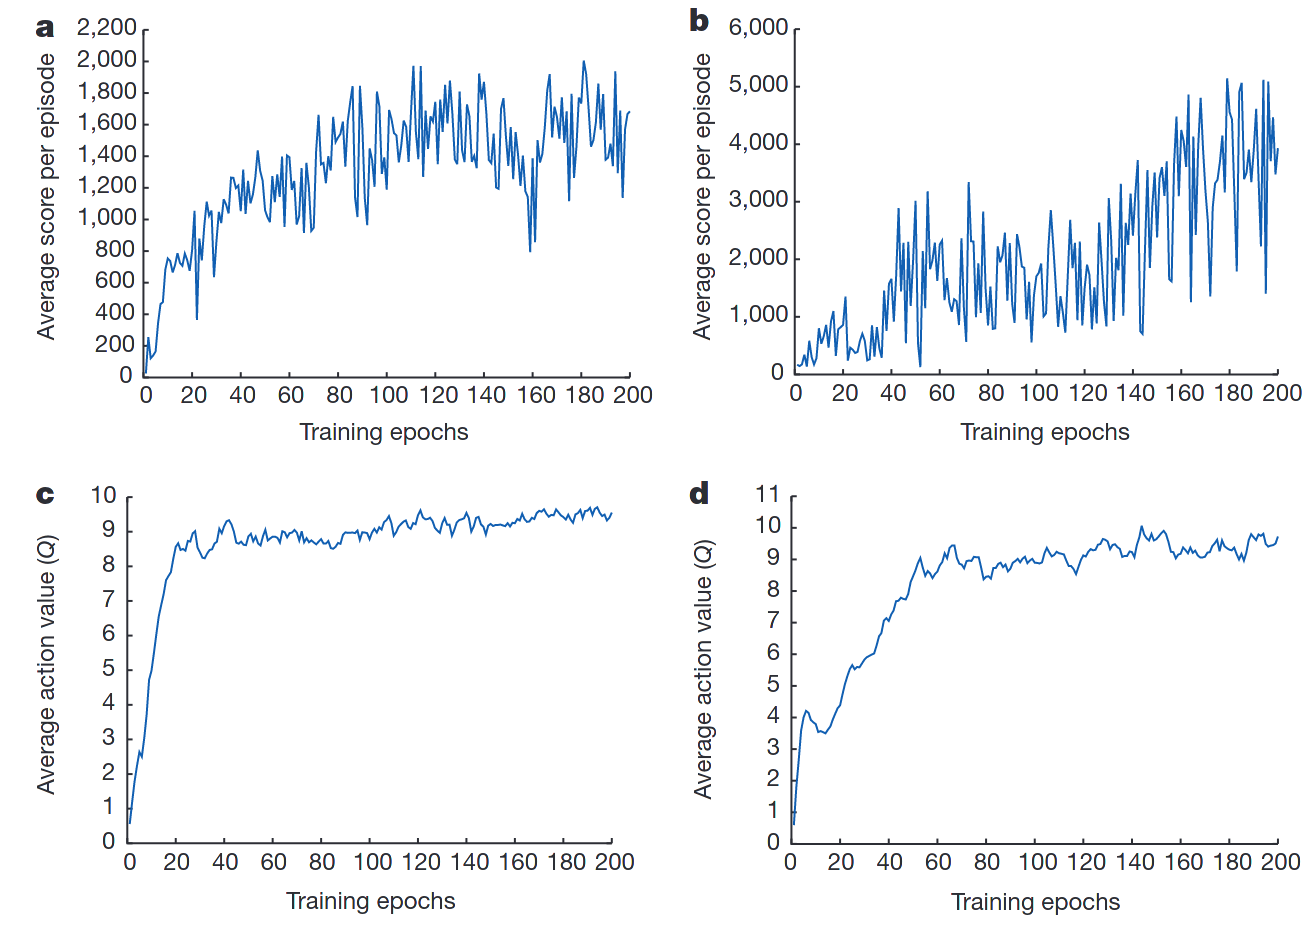
\includegraphics[width=5.cm]{img/Ergebnisse2.png}
      \caption*{\tiny{\textbf{Quelle:} V. Mnih, \url{https://www.nature.com/articles/nature14236}}}
    \end{figure}
    \center
      \scriptsize{
        Agent spielt Breakout:
        \url{https://www.youtube.com/watch?v=TmPfTpjtdgg}
        }
  \end{minipage}
\end{frame}
%% Tell them what they have learned

\section{Zusammenfassung}
\begin{frame}
  \frametitle{Wor�ber haben wir gesprochen ?}
  \begin{enumerate}
  \item MDP's am Beispiel Atari
  \item Q-Funktionen
  \item Architektur/NN
  \item DQN-Algorithmus
  \end{enumerate}
\end{frame}

\setbeamertemplate{headline}{}
\begin{frame}
  \vspace{-0.8cm}
  \begin{center}
    \begin{tabular}{cccc}
      \includegraphics[page=3, width=0.2\textwidth]{img/End.pdf} &
      \includegraphics[page=4, width=0.2\textwidth]{img/End.pdf} &
      \includegraphics[page=5, width=0.2\textwidth]{img/End.pdf} &
      \includegraphics[page=7, width=0.2\textwidth]{img/End.pdf} \\

      \includegraphics[page=9, width=0.2\textwidth]{img/End.pdf} &
      \includegraphics[page=11, width=0.2\textwidth]{img/End.pdf} &
      \includegraphics[page=13, width=0.2\textwidth]{img/End.pdf} &
      \includegraphics[page=17, width=0.2\textwidth]{img/End.pdf} \\

      \includegraphics[page=18, width=0.2\textwidth]{img/End.pdf} &
      \includegraphics[page=19, width=0.2\textwidth]{img/End.pdf} &
      \includegraphics[page=21, width=0.2\textwidth]{img/End.pdf} &
      \includegraphics[page=23, width=0.2\textwidth]{img/End.pdf} \\
    \end{tabular}
    
    \begin{tabular}{cc}
      \includegraphics[page=24, width=0.2\textwidth]{img/End.pdf} &
      \includegraphics[page=26, width=0.2\textwidth]{img/End.pdf}\\
    \end{tabular}
  \end{center}
  \begin{block}{}
    \centering Danke f�r Ihre Aufmerksamkeit.\\
    Gibt es Fragen ?
  \end{block}
\end{frame}

\setbeamertemplate{headline}
{\begin{minipage}[c][0.9cm]{\paperwidth}
		\begin{minipage}{0.2\paperwidth}
		  \centering
                  %% Logo can be changed
			
\includegraphics[width=0.15\paperwidth]{img/FH_Dortmund-logo.png}
		\end{minipage}
		\begin{minipage}{0.8\paperwidth}
		%F�gt die Standard-Navi ein (miniframes)
		  \insertnavigation{0.75\paperwidth}
			\vskip4pt
		\end{minipage}
	\end{minipage}
	\color{DarkCyan}\rule{\paperwidth}{5pt} 
}

\begin{frame}%
  \frametitle{Quellen}
  \begin{thebibliography}{}
    \setbeamertemplate{bibliography item}[book]
    \scriptsize{
    \bibitem[Sutton, 2018]{SuttonRL}\textcolor{red}{R.S.~Sutton, A.G.~Barto}
      \newblock Reinforcement Learning: An Introduction - Chap. 3
      \newblock {\em MIT Press, Cambridge, MA, 2018}
      \newblock \url{http://incompleteideas.net/book/the-book-2nd.html}
      %% Article
      \setbeamertemplate{bibliography item}[article]
    \bibitem[Brockman, 2016]{Brockman2016} \textcolor{red}{G.~Brockman, V.~Cheung, L.~Pettersson, J.~Schneider, J.~Schulman, J.~Tang, W.~Zaremba}
      \newblock OpenAI Gym
      \newblock {\em arXiv:1606.01540, 2016}
      \newblock \url{https://arxiv.org/abs/1606.01540}
    \bibitem[Bellemare, 2013]{Bellemare2013} \textcolor{red}{M.G.~Bellemare, Y.~Naddaf, J.~Veness, M.~Bowling}
      \newblock The Arcade Learning Environment: An Evaluation Platform for General Agents
      \newblock {\em arXiv:1207.4708, 2013}
      \newblock \url{https://arxiv.org/abs/1207.4708}
    \bibitem[Mnih, 2013]{Mnih2013} \textcolor{red}{V.~Mnih, K.~Kavukcuoglu, D.~Silver, A.~Graves,I.~Antonoglou, D.~Wierstra, M.~Riedmiller}
      \newblock Playing Atari with Deep Reinforcement Learning
      \newblock {\em arXiv:1312.5602, 2013}
      \newblock \url{https://arxiv.org/abs/1312.5602}
       \bibitem[Mnih, 2015]{Mnih2015} \textcolor{red}{V.~Mnih, K.~Kavukcuoglu, D.~Silver, A.~Graves,I.~Antonoglou, D.~Wierstra, M.~Riedmiller, \dots}
      \newblock Human-level control through deep reinforcement learning
      \newblock {\em Nature 518, 529-533 (2015)}
      \newblock \tiny{\url{https://storage.googleapis.com/deepmind-media/dqn/DQNNaturePaper.pdf}}
    }
      %\setbeamertemplate{bibliography item}[online]
  \end{thebibliography}
\end{frame}
\begin{frame}
  \frametitle{Quellen}
  \begin{thebibliography}{}
    \setbeamertemplate{bibliography item}[online]
    \scriptsize{
  \bibitem[DanielS, 2016]{Daniel2016}\textcolor{red}{D.~Seita}
    \newblock Frame Skipping and Pre-Processing for Deep Q-Networks on Atari 2600 Games
    \newblock {\tiny{\url{https://danieltakeshi.github.io/2016/11/25/frame-skipping-and-preprocessing-for-deep-q-networks-on-atari-2600-games/}}}
    }
  \end{thebibliography}
  \scriptsize{
    \center Abbildungen:
    \url{https://commons.wikimedia.org/wiki/File:Atari_logo_alt.svg}
    \url{https://de.wikipedia.org/wiki/Datei:Atari-2600-Wood-4Sw-Set.png}
  }
\end{frame}

\end{document}%
